\chapter{Software Architecture}\label{software_architecture}

\begin{figure}[h]
       \centering
       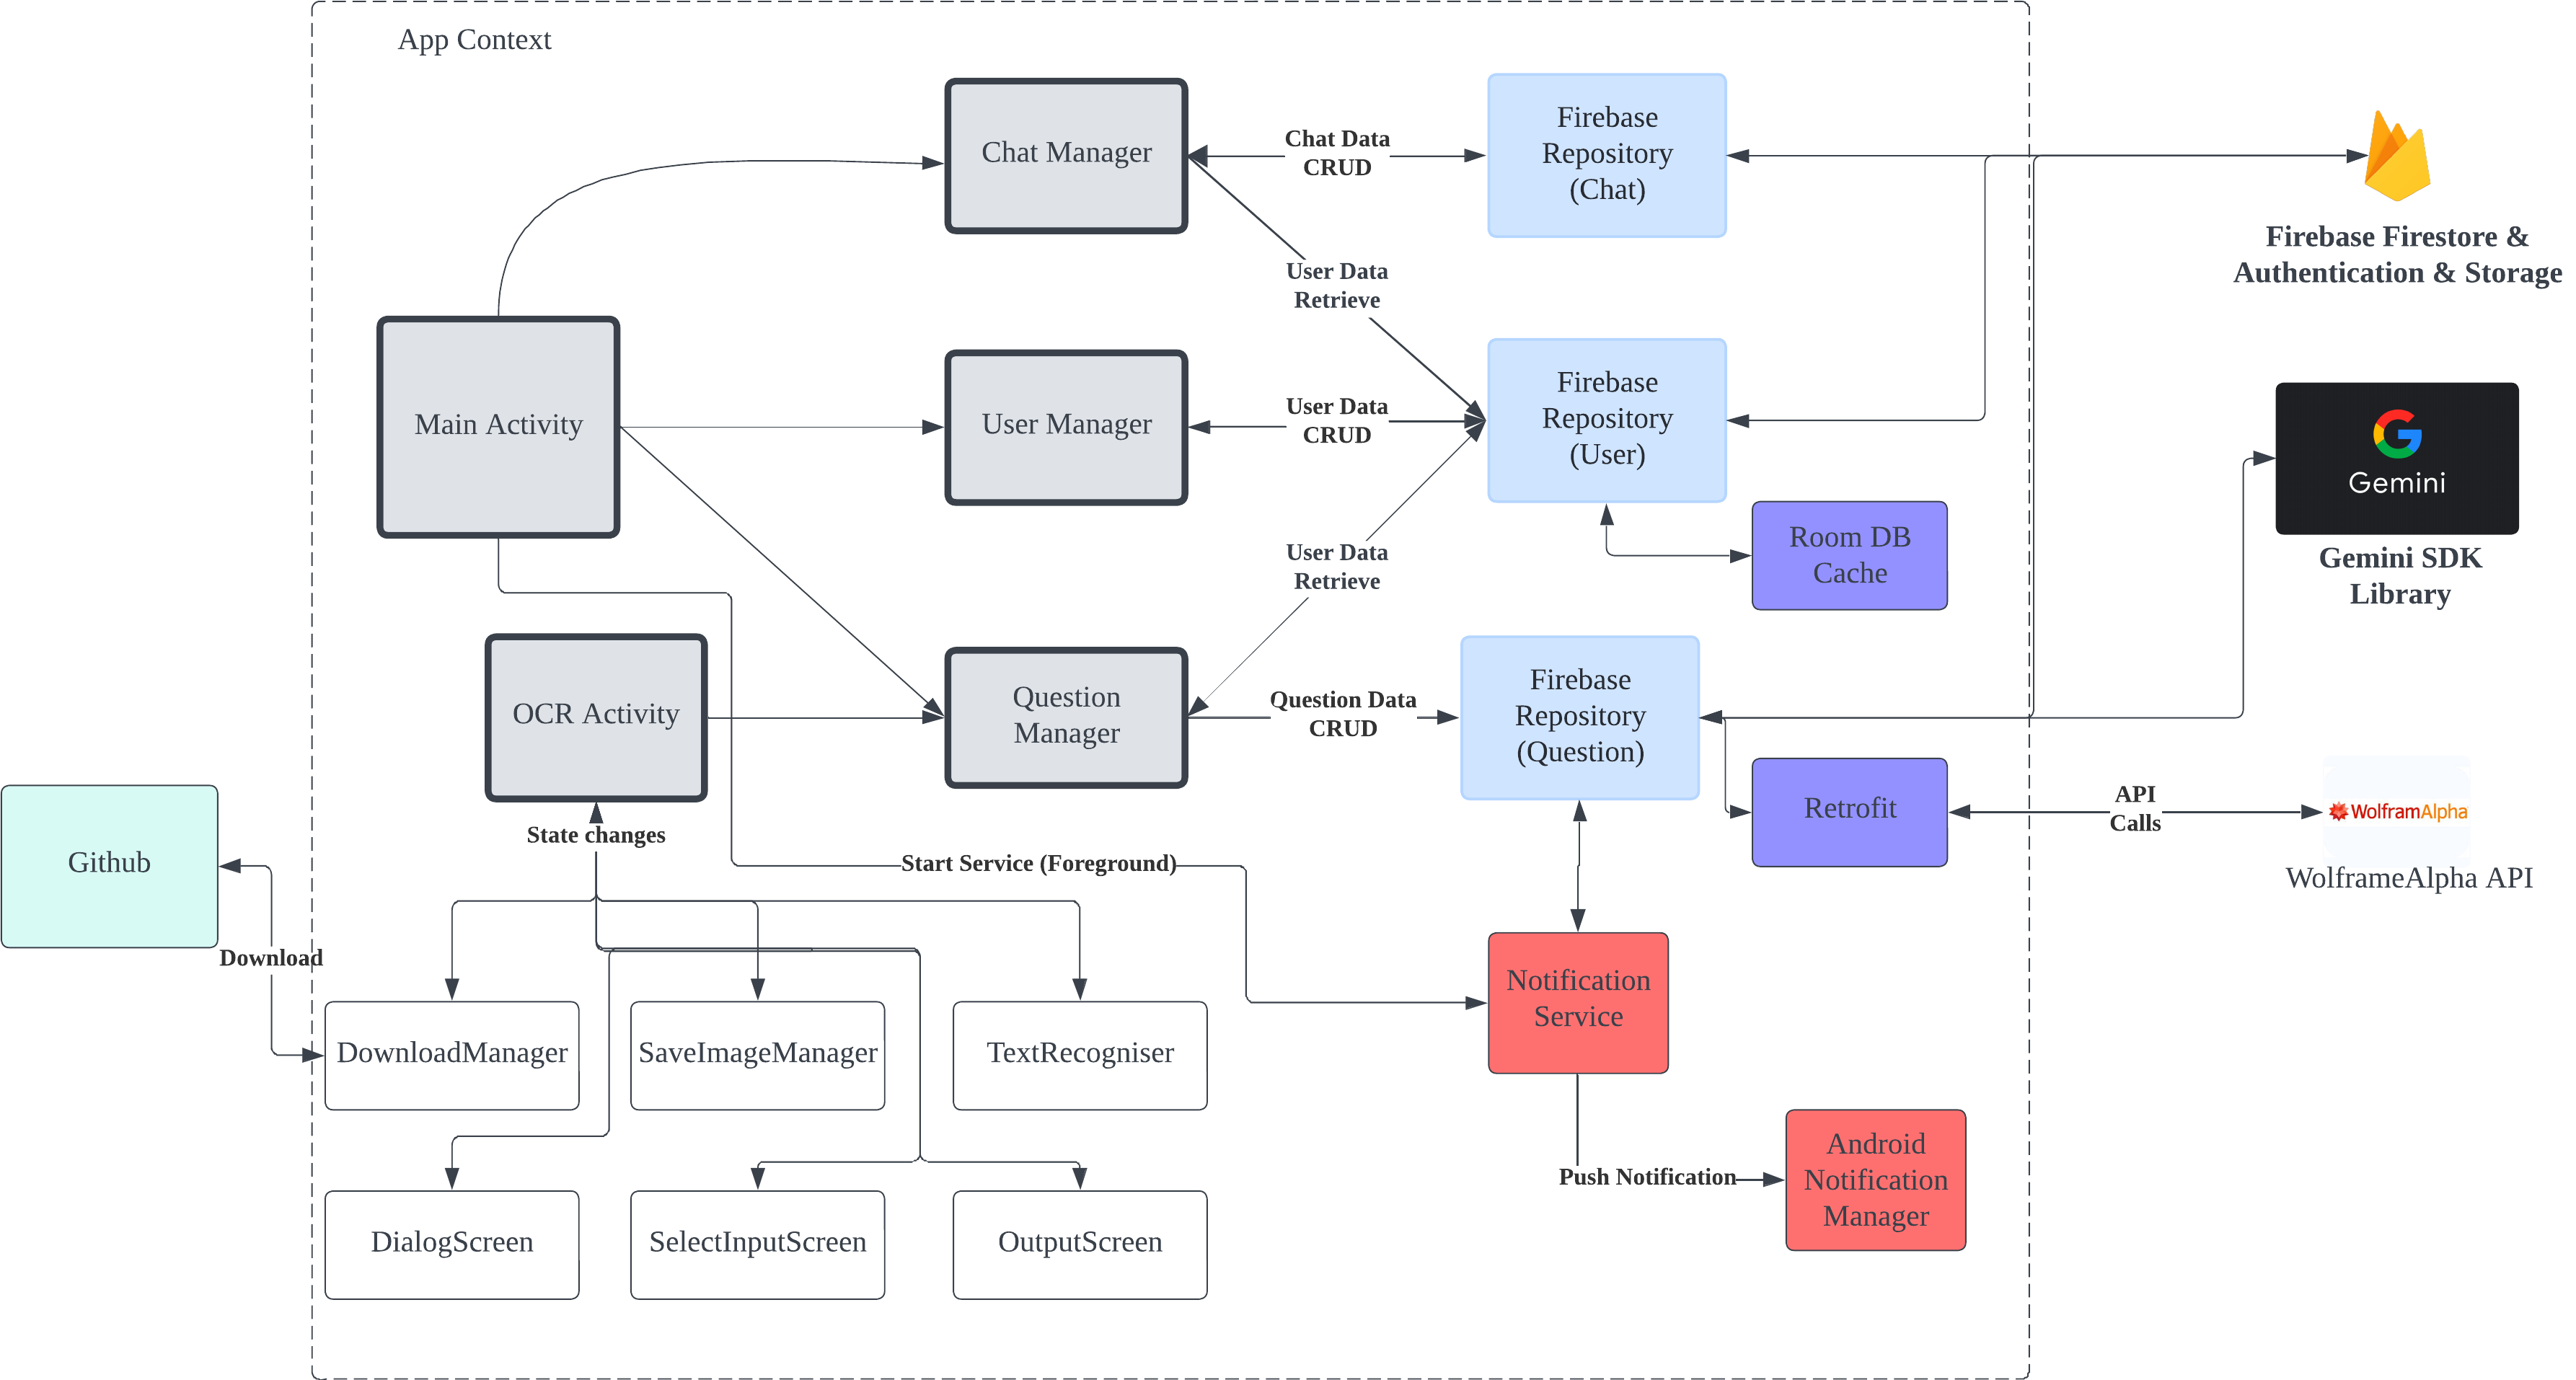
\includegraphics[scale = .80]{Figures/StudyTogether_Architecture.png}
       \caption{\footnotesize Initial Software Architecture}
       \label{StudyTogether_Architecture}
\end{figure}

The diagram illustrates the software architecture designed for our Android application "Study Together." The application leverages the Firebase SDK to access its Authentication and Database services. Additionally, it utilizes a SQLite database to establish and maintain a local cache derived from the Firebase Database, enhancing the overall performance of the application.

The core of our application is the QuestionManager Package, which encapsulates the core functionality related to questions and answers within the program. This component integrates with Google's Gemini AI API to generate potential answers for user queries and also contains functionality for other users to upload and vote on recommended answers. Moreover, an OcrManager component is incorporated, featuring an Optical Character Recognition (OCR) library. This facilitates the extraction of text or questions from images captured by the camera, enabling users to upload questions seamlessly.
